\documentclass[a4paper,12pt,twoside]{article}\usepackage[]{graphicx}\usepackage[]{color}
%% maxwidth is the original width if it is less than linewidth
%% otherwise use linewidth (to make sure the graphics do not exceed the margin)
\makeatletter
\def\maxwidth{ %
  \ifdim\Gin@nat@width>\linewidth
    \linewidth
  \else
    \Gin@nat@width
  \fi
}
\makeatother

\definecolor{fgcolor}{rgb}{0.345, 0.345, 0.345}
\newcommand{\hlnum}[1]{\textcolor[rgb]{0.686,0.059,0.569}{#1}}%
\newcommand{\hlstr}[1]{\textcolor[rgb]{0.192,0.494,0.8}{#1}}%
\newcommand{\hlcom}[1]{\textcolor[rgb]{0.678,0.584,0.686}{\textit{#1}}}%
\newcommand{\hlopt}[1]{\textcolor[rgb]{0,0,0}{#1}}%
\newcommand{\hlstd}[1]{\textcolor[rgb]{0.345,0.345,0.345}{#1}}%
\newcommand{\hlkwa}[1]{\textcolor[rgb]{0.161,0.373,0.58}{\textbf{#1}}}%
\newcommand{\hlkwb}[1]{\textcolor[rgb]{0.69,0.353,0.396}{#1}}%
\newcommand{\hlkwc}[1]{\textcolor[rgb]{0.333,0.667,0.333}{#1}}%
\newcommand{\hlkwd}[1]{\textcolor[rgb]{0.737,0.353,0.396}{\textbf{#1}}}%
\let\hlipl\hlkwb

\usepackage{framed}
\makeatletter
\newenvironment{kframe}{%
 \def\at@end@of@kframe{}%
 \ifinner\ifhmode%
  \def\at@end@of@kframe{\end{minipage}}%
  \begin{minipage}{\columnwidth}%
 \fi\fi%
 \def\FrameCommand##1{\hskip\@totalleftmargin \hskip-\fboxsep
 \colorbox{shadecolor}{##1}\hskip-\fboxsep
     % There is no \\@totalrightmargin, so:
     \hskip-\linewidth \hskip-\@totalleftmargin \hskip\columnwidth}%
 \MakeFramed {\advance\hsize-\width
   \@totalleftmargin\z@ \linewidth\hsize
   \@setminipage}}%
 {\par\unskip\endMakeFramed%
 \at@end@of@kframe}
\makeatother

\definecolor{shadecolor}{rgb}{.97, .97, .97}
\definecolor{messagecolor}{rgb}{0, 0, 0}
\definecolor{warningcolor}{rgb}{1, 0, 1}
\definecolor{errorcolor}{rgb}{1, 0, 0}
\newenvironment{knitrout}{}{} % an empty environment to be redefined in TeX

\usepackage{alltt}
\usepackage[margin=2cm]{geometry}
\usepackage{placeins}
\usepackage{graphicx}
\usepackage{color}
\usepackage{hyperref}
\title{Exp 2 of 4}
\IfFileExists{upquote.sty}{\usepackage{upquote}}{}
\begin{document}



\maketitle
\tableofcontents
\clearpage





\section{Get the data}

\begin{knitrout}\scriptsize
\definecolor{shadecolor}{rgb}{0.969, 0.969, 0.969}\color{fgcolor}\begin{kframe}
\begin{alltt}
\hlkwd{source}\hlstd{(}\hlstr{"e2-preprocessing.R"}\hlstd{)}
\hlkwa{if} \hlstd{(}\hlopt{!}\hlkwd{file.exists}\hlstd{(}\hlstr{"e2-b-data.txt"}\hlstd{)) \{}
    \hlstd{dat} \hlkwb{<-} \hlkwd{gatherData}\hlstd{()}
    \hlstd{dat} \hlkwb{<-} \hlkwd{declareImpossibleRT}\hlstd{(dat)}
    \hlstd{dat} \hlkwb{<-} \hlkwd{removeImpossibleTrials}\hlstd{(dat)}
    \hlstd{dat} \hlkwb{<-} \hlkwd{subset}\hlstd{(dat,} \hlkwc{select} \hlstd{=} \hlkwd{c}\hlstd{(Subject, Trial, Item, discriminability, Instruction, nchar_instr, Vagueness,}
        \hlstd{Number, Order, Quantity, c_Vag, c_Num, c_Ord, c_Qty, NaType, response_category, isBorderline,}
        \hlstd{RT))}
    \hlkwd{write.table}\hlstd{(dat,} \hlkwc{file} \hlstd{=} \hlstr{"e2-b-data.txt"}\hlstd{,} \hlkwc{sep} \hlstd{=} \hlstr{"\textbackslash{}t"}\hlstd{,} \hlkwc{quote} \hlstd{=} \hlnum{FALSE}\hlstd{)}
\hlstd{\}}
\hlstd{dat} \hlkwb{<-} \hlkwd{read.delim}\hlstd{(}\hlstr{"e2-b-data.txt"}\hlstd{)}
\hlstd{dd} \hlkwb{<-} \hlkwd{read.delim}\hlstd{(}\hlstr{"e2-b-data.txt"}\hlstd{)}
\end{alltt}
\end{kframe}
\end{knitrout}

\clearpage

\begin{knitrout}\scriptsize
\definecolor{shadecolor}{rgb}{0.969, 0.969, 0.969}\color{fgcolor}\begin{kframe}
\begin{alltt}
\hlkwd{names}\hlstd{(dd)}
\end{alltt}
\begin{verbatim}
 [1] "Subject"           "Trial"             "Item"              "discriminability" 
 [5] "Instruction"       "nchar_instr"       "Vagueness"         "Number"           
 [9] "Order"             "Quantity"          "c_Vag"             "c_Num"            
[13] "c_Ord"             "c_Qty"             "NaType"            "response_category"
[17] "isBorderline"      "RT"               
\end{verbatim}
\end{kframe}
\end{knitrout}

\clearpage

\begin{knitrout}\scriptsize
\definecolor{shadecolor}{rgb}{0.969, 0.969, 0.969}\color{fgcolor}\begin{kframe}
\begin{alltt}
\hlkwd{head}\hlstd{(dd)}
\end{alltt}
\begin{verbatim}
  Subject Trial     Item discriminability                            Instruction nchar_instr
1     s01     1 06:15:24        0.4875000          Choose the square with 6 dots          29
2     s01     2 16:25:34        0.3123529     Choose a square with about 30 dots          34
3     s01     3 26:35:44        0.2308442 Choose the square with the fewest dots          38
4     s01     4 36:45:54        0.1833333     Choose a square with about 50 dots          34
5     s01     5 06:15:24        0.4875000     Choose a square with about 10 dots          34
6     s01     6 16:25:34        0.3123529         Choose a square with many dots          30
  Vagueness  Number Order Quantity c_Vag c_Num c_Ord c_Qty      NaType response_category
1     Crisp Numeric  RtoL    Small  -0.5  -0.5   0.5  -0.5 valid_trial          expected
2     Vague Numeric  LtoR    Large   0.5  -0.5  -0.5   0.5 valid_trial        borderline
3     Crisp  Verbal  LtoR    Small  -0.5   0.5  -0.5  -0.5 valid_trial          expected
4     Vague Numeric  RtoL    Large   0.5  -0.5   0.5   0.5 valid_trial        borderline
5     Vague Numeric  RtoL    Small   0.5  -0.5   0.5  -0.5 valid_trial          expected
6     Vague  Verbal  LtoR    Large   0.5   0.5  -0.5   0.5 valid_trial          expected
  isBorderline   RT
1        FALSE 1517
2         TRUE 1920
3        FALSE 2346
4         TRUE 1773
5        FALSE 2556
6        FALSE 2043
\end{verbatim}
\end{kframe}
\end{knitrout}

\clearpage

\begin{knitrout}\scriptsize
\definecolor{shadecolor}{rgb}{0.969, 0.969, 0.969}\color{fgcolor}\begin{kframe}
\begin{alltt}
\hlkwd{summary}\hlstd{(dd)}
\end{alltt}
\begin{verbatim}
    Subject         Trial             Item      discriminability
 s01    : 256   Min.   :  1.0   06:15:24:1919   Min.   :0.1833  
 s02    : 256   1st Qu.: 65.0   16:25:34:1919   1st Qu.:0.2308  
 s03    : 256   Median :129.0   26:35:44:1920   Median :0.2308  
 s04    : 256   Mean   :128.5   36:45:54:1919   Mean   :0.3035  
 s05    : 256   3rd Qu.:193.0                   3rd Qu.:0.3124  
 s06    : 256   Max.   :256.0                   Max.   :0.4875  
 (Other):6141                                                   
                                 Instruction    nchar_instr    Vagueness        Number    
 Choose a square with few dots         : 960   Min.   :29.00   Crisp:3840   Numeric:3838  
 Choose the square with the fewest dots: 960   1st Qu.:30.00   Vague:3837   Verbal :3839  
 Choose the square with the most dots  : 960   Median :30.00                              
 Choose a square with many dots        : 959   Mean   :32.59                              
 Choose a square with about 30 dots    : 480   3rd Qu.:36.00                              
 Choose a square with about 40 dots    : 480   Max.   :38.00                              
 (Other)                               :2878                                              
  Order       Quantity        c_Vag                c_Num               c_Ord          
 LtoR:3838   Large:3837   Min.   :-0.5000000   Min.   :-5.00e-01   Min.   :-5.00e-01  
 RtoL:3839   Small:3840   1st Qu.:-0.5000000   1st Qu.:-5.00e-01   1st Qu.:-5.00e-01  
                          Median :-0.5000000   Median : 5.00e-01   Median : 5.00e-01  
                          Mean   :-0.0001954   Mean   : 6.51e-05   Mean   : 6.51e-05  
                          3rd Qu.: 0.5000000   3rd Qu.: 5.00e-01   3rd Qu.: 5.00e-01  
                          Max.   : 0.5000000   Max.   : 5.00e-01   Max.   : 5.00e-01  
                                                                                      
     c_Qty                    NaType      response_category isBorderline          RT       
 Min.   :-0.5000000   valid_trial:7677   borderline:1274    Mode :logical   Min.   :  445  
 1st Qu.:-0.5000000                      expected  :6108    FALSE:6403      1st Qu.: 1240  
 Median :-0.5000000                      extreme   : 295    TRUE :1274      Median : 1727  
 Mean   :-0.0001954                                         NA's :0         Mean   : 2840  
 3rd Qu.: 0.5000000                                                         3rd Qu.: 2699  
 Max.   : 0.5000000                                                         Max.   :42685  
                                                                                           
\end{verbatim}
\end{kframe}
\end{knitrout}

\clearpage

\begin{knitrout}\scriptsize
\definecolor{shadecolor}{rgb}{0.969, 0.969, 0.969}\color{fgcolor}\begin{kframe}
\begin{alltt}
\hlkwd{str}\hlstd{(dd)}
\end{alltt}
\begin{verbatim}
'data.frame':	7677 obs. of  18 variables:
 $ Subject          : Factor w/ 30 levels "s01","s02","s03",..: 1 1 1 1 1 1 1 1 1 1 ...
 $ Trial            : int  1 2 3 4 5 6 7 8 9 10 ...
 $ Item             : Factor w/ 4 levels "06:15:24","16:25:34",..: 1 2 3 4 1 2 3 4 1 2 ...
 $ discriminability : num  0.487 0.312 0.231 0.183 0.487 ...
 $ Instruction      : Factor w/ 17 levels "Choose a square with about 10 dots",..: 15 3 16 5 1 7 6 16 17 11 ...
 $ nchar_instr      : int  29 34 38 34 34 30 29 38 36 30 ...
 $ Vagueness        : Factor w/ 2 levels "Crisp","Vague": 1 2 1 2 2 2 2 1 1 1 ...
 $ Number           : Factor w/ 2 levels "Numeric","Verbal": 1 1 2 1 1 2 2 2 2 1 ...
 $ Order            : Factor w/ 2 levels "LtoR","RtoL": 2 1 1 2 2 1 2 2 1 2 ...
 $ Quantity         : Factor w/ 2 levels "Large","Small": 2 1 2 1 2 1 2 2 1 1 ...
 $ c_Vag            : num  -0.5 0.5 -0.5 0.5 0.5 0.5 0.5 -0.5 -0.5 -0.5 ...
 $ c_Num            : num  -0.5 -0.5 0.5 -0.5 -0.5 0.5 0.5 0.5 0.5 -0.5 ...
 $ c_Ord            : num  0.5 -0.5 -0.5 0.5 0.5 -0.5 0.5 0.5 -0.5 0.5 ...
 $ c_Qty            : num  -0.5 0.5 -0.5 0.5 -0.5 0.5 -0.5 -0.5 0.5 0.5 ...
 $ NaType           : Factor w/ 1 level "valid_trial": 1 1 1 1 1 1 1 1 1 1 ...
 $ response_category: Factor w/ 3 levels "borderline","expected",..: 2 1 2 1 2 2 2 2 2 1 ...
 $ isBorderline     : logi  FALSE TRUE FALSE TRUE FALSE FALSE ...
 $ RT               : int  1517 1920 2346 1773 2556 2043 2384 3078 1760 2218 ...
\end{verbatim}
\end{kframe}
\end{knitrout}

\clearpage
\section{Plots}
\clearpage
\subsection{Discriminability}

\begin{knitrout}\scriptsize
\definecolor{shadecolor}{rgb}{0.969, 0.969, 0.969}\color{fgcolor}\begin{figure}[hbtp]

{\centering 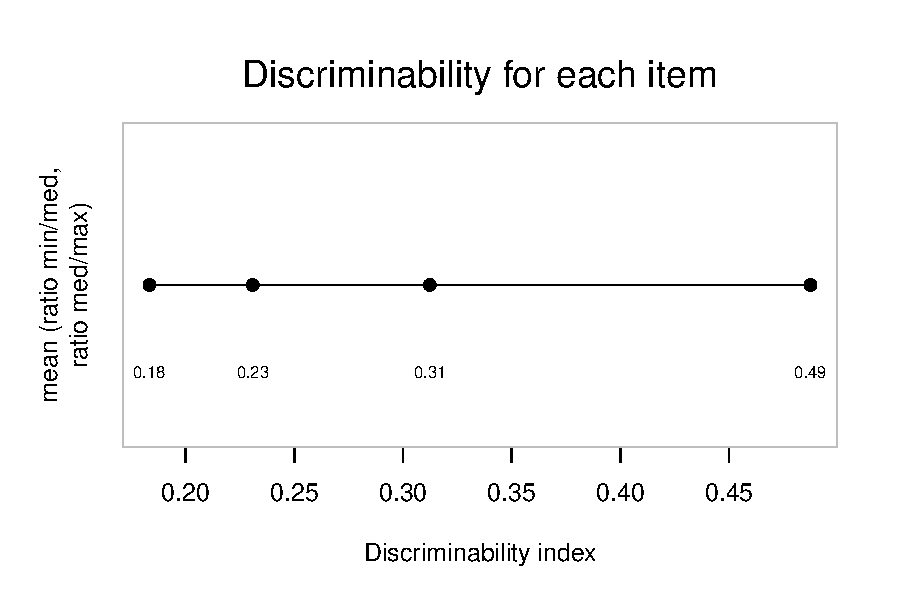
\includegraphics[width=\maxwidth]{figure/graphics-showCompression-1} 

}

\caption[Ratios for different numbers of dots in the arrays]{Ratios for different numbers of dots in the arrays: smaller values are more discriminable. Blue is for the ratio between the smallest number in the array and the largest number in an array. Red is for the mean of two ratios, one for the smallest number to the middle number, the other for the middle number to the largest number in the array}\label{fig:showCompression}
\end{figure}


\end{knitrout}

\clearpage
\subsection{Consider using log RT}

\begin{knitrout}\scriptsize
\definecolor{shadecolor}{rgb}{0.969, 0.969, 0.969}\color{fgcolor}\begin{kframe}


{\ttfamily\noindent\bfseries\color{errorcolor}{Error in `*tmp*`[[j]]: subscript out of bounds}}

{\ttfamily\noindent\color{warningcolor}{Warning in mean.default(dat\_transforms[dat\_transforms\$dfSubset == k \& dat\_transforms\$RTtype == : argument is not numeric or logical: returning NA}}

{\ttfamily\noindent\bfseries\color{errorcolor}{Error in `[<-.data.frame`(`*tmp*`, dat\_transforms\$dfSubset == k \& dat\_transforms\$RTtype == : replacement has length zero}}\end{kframe}
\end{knitrout}

\begin{knitrout}\scriptsize
\definecolor{shadecolor}{rgb}{0.969, 0.969, 0.969}\color{fgcolor}\begin{kframe}


{\ttfamily\noindent\bfseries\color{errorcolor}{Error: measure variables not found in data: RT\_log, RT\_raw}}

{\ttfamily\noindent\bfseries\color{errorcolor}{Error in ggplot(temp, aes(time, colour = RTtype)): object 'temp' not found}}\end{kframe}
\end{knitrout}

\clearpage
\subsection{How logging RT affects the distribution}


\begin{knitrout}\scriptsize
\definecolor{shadecolor}{rgb}{0.969, 0.969, 0.969}\color{fgcolor}\begin{kframe}


{\ttfamily\noindent\color{warningcolor}{Warning in readChar(con, 5L, useBytes = TRUE): cannot open compressed file 'data\_processed.Rda', probable reason 'No such file or directory'}}

{\ttfamily\noindent\bfseries\color{errorcolor}{Error in readChar(con, 5L, useBytes = TRUE): cannot open the connection}}

{\ttfamily\noindent\bfseries\color{errorcolor}{Error: measure variables not found in data: RT\_log, RT\_raw}}

{\ttfamily\noindent\bfseries\color{errorcolor}{Error in ggplot(subdata): object 'subdata' not found}}\end{kframe}
\end{knitrout}

\clearpage
\subsection{Identify fast and slow subjects and items}


\begin{knitrout}\scriptsize
\definecolor{shadecolor}{rgb}{0.969, 0.969, 0.969}\color{fgcolor}\begin{kframe}


{\ttfamily\noindent\color{warningcolor}{Warning in mean.default(dd\$RT\_log): argument is not numeric or logical: returning NA}}

{\ttfamily\noindent\bfseries\color{errorcolor}{Error in mean(RT\_log): object 'RT\_log' not found}}

{\ttfamily\noindent\bfseries\color{errorcolor}{Error in subs\$level = 1:30: object 'subs' not found}}

{\ttfamily\noindent\bfseries\color{errorcolor}{Error in factor(subs\$effect, levels = c("{}subject"{}, "{}discriminability"{})): object 'subs' not found}}

{\ttfamily\noindent\color{warningcolor}{Warning in mean.default(dd\$RT\_log): argument is not numeric or logical: returning NA}}

{\ttfamily\noindent\bfseries\color{errorcolor}{Error in mean(RT\_log): object 'RT\_log' not found}}

{\ttfamily\noindent\bfseries\color{errorcolor}{Error in factor(itms\$effect, levels = c("{}subject"{}, "{}discriminability"{})): object 'itms' not found}}

{\ttfamily\noindent\bfseries\color{errorcolor}{Error in rbind(subs, itms): object 'subs' not found}}

{\ttfamily\noindent\bfseries\color{errorcolor}{Error in factor(si\$effect, levels = c("{}subject"{}, "{}discriminability"{})): object 'si' not found}}

{\ttfamily\noindent\bfseries\color{errorcolor}{Error in unique(si\$emean): object 'si' not found}}

{\ttfamily\noindent\bfseries\color{errorcolor}{Error in eval(substitute(groups), data, environment(x)): object 'si' not found}}

{\ttfamily\noindent\bfseries\color{errorcolor}{Error in inherits(obj1, "{}trellis"{}): object 'my1' not found}}\end{kframe}
\end{knitrout}

\clearpage
\subsection{Plot main effects in both transformations}


\begin{knitrout}\scriptsize
\definecolor{shadecolor}{rgb}{0.969, 0.969, 0.969}\color{fgcolor}\begin{kframe}


{\ttfamily\noindent\bfseries\color{errorcolor}{Error: measure variables not found in data: RT\_raw}}

{\ttfamily\noindent\bfseries\color{errorcolor}{Error in reshape2::melt(tempraw, id.vars = c("{}transformation"{}, "{}score"{}), : object 'tempraw' not found}}

{\ttfamily\noindent\bfseries\color{errorcolor}{Error: measure variables not found in data: RT\_log}}

{\ttfamily\noindent\bfseries\color{errorcolor}{Error in reshape2::melt(templog, id.vars = c("{}transformation"{}, "{}score"{}), : object 'templog' not found}}\end{kframe}
\end{knitrout}
  
\begin{knitrout}\scriptsize
\definecolor{shadecolor}{rgb}{0.969, 0.969, 0.969}\color{fgcolor}\begin{kframe}


{\ttfamily\noindent\bfseries\color{errorcolor}{Error in ggplot(tempraw2, aes(y = score, x = level, group = 1, col = effect)): object 'tempraw2' not found}}\end{kframe}
\end{knitrout}
  
\begin{knitrout}\scriptsize
\definecolor{shadecolor}{rgb}{0.969, 0.969, 0.969}\color{fgcolor}\begin{kframe}


{\ttfamily\noindent\bfseries\color{errorcolor}{Error in ggplot(templog2, aes(y = score, x = level, group = 1, col = effect)): object 'templog2' not found}}\end{kframe}
\end{knitrout}
  
\clearpage
\subsection{Main effects in log RT over discriminability}


\begin{knitrout}\scriptsize
\definecolor{shadecolor}{rgb}{0.969, 0.969, 0.969}\color{fgcolor}\begin{kframe}


{\ttfamily\noindent\bfseries\color{errorcolor}{Error in `[.data.frame`(xx, , col): undefined columns selected}}

{\ttfamily\noindent\bfseries\color{errorcolor}{Error in names(nrts)[5] <- "{}Levels"{}: object 'nrts' not found}}

{\ttfamily\noindent\bfseries\color{errorcolor}{Error in `[.data.frame`(xx, , col): undefined columns selected}}

{\ttfamily\noindent\bfseries\color{errorcolor}{Error in names(orts)[5] <- "{}Levels"{}: object 'orts' not found}}

{\ttfamily\noindent\bfseries\color{errorcolor}{Error in `[.data.frame`(xx, , col): undefined columns selected}}

{\ttfamily\noindent\bfseries\color{errorcolor}{Error in names(qrts)[5] <- "{}Levels"{}: object 'qrts' not found}}

{\ttfamily\noindent\bfseries\color{errorcolor}{Error in `[.data.frame`(xx, , col): undefined columns selected}}

{\ttfamily\noindent\bfseries\color{errorcolor}{Error in names(vrts)[5] <- "{}Levels"{}: object 'vrts' not found}}

{\ttfamily\noindent\bfseries\color{errorcolor}{Error in rbind(nrts, orts, qrts, vrts): object 'nrts' not found}}

{\ttfamily\noindent\bfseries\color{errorcolor}{Error in eval(expr, envir, enclos): object 'rts' not found}}

{\ttfamily\noindent\bfseries\color{errorcolor}{Error in eval(expr, envir, enclos): object 'rts' not found}}

{\ttfamily\noindent\bfseries\color{errorcolor}{Error in eval(expr, envir, enclos): object 'rts' not found}}

{\ttfamily\noindent\bfseries\color{errorcolor}{Error in ggplot(data = rts, aes(x = discriminability, y = RT\_log, group = Levels)): object 'rts' not found}}

{\ttfamily\noindent\bfseries\color{errorcolor}{Error in eval(expr, envir, enclos): object 'p1' not found}}\end{kframe}
\end{knitrout}

\clearpage
\subsection{2-Way interactions over discriminability}


\begin{knitrout}\scriptsize
\definecolor{shadecolor}{rgb}{0.969, 0.969, 0.969}\color{fgcolor}\begin{kframe}


{\ttfamily\noindent\bfseries\color{errorcolor}{Error in `[.data.frame`(xx, , col): undefined columns selected}}

{\ttfamily\noindent\bfseries\color{errorcolor}{Error in names(rts1)[2] <- "{}F1"{}: object 'rts1' not found}}

{\ttfamily\noindent\bfseries\color{errorcolor}{Error in names(rts1)[3] <- "{}F2"{}: object 'rts1' not found}}

{\ttfamily\noindent\bfseries\color{errorcolor}{Error in rts1\$E1 <- "{}Vagueness"{}: object 'rts1' not found}}

{\ttfamily\noindent\bfseries\color{errorcolor}{Error in rts1\$E2 <- "{}Number"{}: object 'rts1' not found}}

{\ttfamily\noindent\bfseries\color{errorcolor}{Error in `[.data.frame`(xx, , col): undefined columns selected}}

{\ttfamily\noindent\bfseries\color{errorcolor}{Error in names(rts2)[2] <- "{}F1"{}: object 'rts2' not found}}

{\ttfamily\noindent\bfseries\color{errorcolor}{Error in names(rts2)[3] <- "{}F2"{}: object 'rts2' not found}}

{\ttfamily\noindent\bfseries\color{errorcolor}{Error in rts2\$E1 <- "{}Vagueness"{}: object 'rts2' not found}}

{\ttfamily\noindent\bfseries\color{errorcolor}{Error in rts2\$E2 <- "{}Quantity"{}: object 'rts2' not found}}

{\ttfamily\noindent\bfseries\color{errorcolor}{Error in `[.data.frame`(xx, , col): undefined columns selected}}

{\ttfamily\noindent\bfseries\color{errorcolor}{Error in names(rts3)[2] <- "{}F1"{}: object 'rts3' not found}}

{\ttfamily\noindent\bfseries\color{errorcolor}{Error in names(rts3)[3] <- "{}F2"{}: object 'rts3' not found}}

{\ttfamily\noindent\bfseries\color{errorcolor}{Error in rts3\$E1 <- "{}Vagueness"{}: object 'rts3' not found}}

{\ttfamily\noindent\bfseries\color{errorcolor}{Error in rts3\$E2 <- "{}Order"{}: object 'rts3' not found}}

{\ttfamily\noindent\bfseries\color{errorcolor}{Error in `[.data.frame`(xx, , col): undefined columns selected}}

{\ttfamily\noindent\bfseries\color{errorcolor}{Error in names(rts4)[2] <- "{}F1"{}: object 'rts4' not found}}

{\ttfamily\noindent\bfseries\color{errorcolor}{Error in names(rts4)[3] <- "{}F2"{}: object 'rts4' not found}}

{\ttfamily\noindent\bfseries\color{errorcolor}{Error in rts4\$E1 <- "{}Quantity"{}: object 'rts4' not found}}

{\ttfamily\noindent\bfseries\color{errorcolor}{Error in rts4\$E2 <- "{}Number"{}: object 'rts4' not found}}

{\ttfamily\noindent\bfseries\color{errorcolor}{Error in `[.data.frame`(xx, , col): undefined columns selected}}

{\ttfamily\noindent\bfseries\color{errorcolor}{Error in names(rts5)[2] <- "{}F1"{}: object 'rts5' not found}}

{\ttfamily\noindent\bfseries\color{errorcolor}{Error in names(rts5)[3] <- "{}F2"{}: object 'rts5' not found}}

{\ttfamily\noindent\bfseries\color{errorcolor}{Error in rts5\$E1 <- "{}Order"{}: object 'rts5' not found}}

{\ttfamily\noindent\bfseries\color{errorcolor}{Error in rts5\$E2 <- "{}Number"{}: object 'rts5' not found}}

{\ttfamily\noindent\bfseries\color{errorcolor}{Error in `[.data.frame`(xx, , col): undefined columns selected}}

{\ttfamily\noindent\bfseries\color{errorcolor}{Error in names(rts6)[2] <- "{}F1"{}: object 'rts6' not found}}

{\ttfamily\noindent\bfseries\color{errorcolor}{Error in names(rts6)[3] <- "{}F2"{}: object 'rts6' not found}}

{\ttfamily\noindent\bfseries\color{errorcolor}{Error in rts6\$E1 <- "{}Quantity"{}: object 'rts6' not found}}

{\ttfamily\noindent\bfseries\color{errorcolor}{Error in rts6\$E2 <- "{}Order"{}: object 'rts6' not found}}

{\ttfamily\noindent\bfseries\color{errorcolor}{Error in rbind(rts1, rts2, rts3, rts4, rts5, rts6): object 'rts1' not found}}

{\ttfamily\noindent\bfseries\color{errorcolor}{Error in eval(expr, envir, enclos): object 'rts' not found}}

{\ttfamily\noindent\bfseries\color{errorcolor}{Error in eval(expr, envir, enclos): object 'rts' not found}}

{\ttfamily\noindent\bfseries\color{errorcolor}{Error in eval(expr, envir, enclos): object 'rts' not found}}

{\ttfamily\noindent\bfseries\color{errorcolor}{Error in paste(rts\$F1, rts\$F2): object 'rts' not found}}

{\ttfamily\noindent\bfseries\color{errorcolor}{Error in factor(rts\$E1, levels = c("{}Number"{}, "{}Order"{}, "{}Quantity"{}, "{}Vagueness"{})): object 'rts' not found}}

{\ttfamily\noindent\bfseries\color{errorcolor}{Error in factor(rts\$E2, levels = c("{}Number"{}, "{}Order"{}, "{}Quantity"{}, "{}Vagueness"{})): object 'rts' not found}}

{\ttfamily\noindent\bfseries\color{errorcolor}{Error in ggplot(rts, aes(y = RT\_log, x = discriminability, group = F3, : object 'rts' not found}}\end{kframe}
\end{knitrout}

\clearpage
\subsection{Vagueness by number interaction over items}


\begin{knitrout}\scriptsize
\definecolor{shadecolor}{rgb}{0.969, 0.969, 0.969}\color{fgcolor}\begin{kframe}


{\ttfamily\noindent\bfseries\color{errorcolor}{Error in `[.data.frame`(xx, , col): undefined columns selected}}

{\ttfamily\noindent\bfseries\color{errorcolor}{Error in paste(rts\$Number, rts\$Vagueness, sep = "{} "{}): object 'rts' not found}}

{\ttfamily\noindent\bfseries\color{errorcolor}{Error in ggplot(rts, aes(y = RT\_log, x = Item, ymin = RT\_log - ci, ymax = RT\_log + : object 'rts' not found}}\end{kframe}
\end{knitrout}

\clearpage
\subsection{Vagueness by number interaction over discriminability}


\begin{knitrout}\scriptsize
\definecolor{shadecolor}{rgb}{0.969, 0.969, 0.969}\color{fgcolor}\begin{kframe}


{\ttfamily\noindent\bfseries\color{errorcolor}{Error in `[.data.frame`(xx, , col): undefined columns selected}}

{\ttfamily\noindent\bfseries\color{errorcolor}{Error in eval(expr, envir, enclos): object 'rts' not found}}

{\ttfamily\noindent\bfseries\color{errorcolor}{Error in paste(rts\$Number, rts\$Vagueness, sep = "{} "{}): object 'rts' not found}}

{\ttfamily\noindent\bfseries\color{errorcolor}{Error in ggplot(rts, aes(y = RT\_log, x = discriminability, ymin = RT\_log - : object 'rts' not found}}\end{kframe}
\end{knitrout}

\clearpage
\subsection{3-Way interactions}


\begin{knitrout}\scriptsize
\definecolor{shadecolor}{rgb}{0.969, 0.969, 0.969}\color{fgcolor}\begin{kframe}


{\ttfamily\noindent\bfseries\color{errorcolor}{Error in `[.data.frame`(xx, , col): undefined columns selected}}

{\ttfamily\noindent\bfseries\color{errorcolor}{Error in eval(expr, envir, enclos): object 'rts' not found}}

{\ttfamily\noindent\bfseries\color{errorcolor}{Error in eval(expr, envir, enclos): object 'rts' not found}}

{\ttfamily\noindent\bfseries\color{errorcolor}{Error in ggplot(rts, aes(y = RT\_log, x = Number, group = Vagueness, ymin = mins, : object 'rts' not found}}

{\ttfamily\noindent\bfseries\color{errorcolor}{Error in `[.data.frame`(xx, , col): undefined columns selected}}

{\ttfamily\noindent\bfseries\color{errorcolor}{Error in eval(expr, envir, enclos): object 'rts' not found}}

{\ttfamily\noindent\bfseries\color{errorcolor}{Error in eval(expr, envir, enclos): object 'rts' not found}}

{\ttfamily\noindent\bfseries\color{errorcolor}{Error in ggplot(rts, aes(y = RT\_log, x = Number, group = Vagueness, ymin = mins, : object 'rts' not found}}

{\ttfamily\noindent\bfseries\color{errorcolor}{Error in `[.data.frame`(xx, , col): undefined columns selected}}

{\ttfamily\noindent\bfseries\color{errorcolor}{Error in eval(expr, envir, enclos): object 'rts' not found}}

{\ttfamily\noindent\bfseries\color{errorcolor}{Error in eval(expr, envir, enclos): object 'rts' not found}}

{\ttfamily\noindent\bfseries\color{errorcolor}{Error in ggplot(rts, aes(y = RT\_log, x = Number, group = Quantity, ymin = mins, : object 'rts' not found}}

{\ttfamily\noindent\bfseries\color{errorcolor}{Error in `[.data.frame`(xx, , col): undefined columns selected}}

{\ttfamily\noindent\bfseries\color{errorcolor}{Error in eval(expr, envir, enclos): object 'rts' not found}}

{\ttfamily\noindent\bfseries\color{errorcolor}{Error in eval(expr, envir, enclos): object 'rts' not found}}

{\ttfamily\noindent\bfseries\color{errorcolor}{Error in ggplot(rts, aes(y = RT\_log, x = Vagueness, group = Quantity, : object 'rts' not found}}

{\ttfamily\noindent\bfseries\color{errorcolor}{Error in arrangeGrob(...): object 'p1' not found}}\end{kframe}
\end{knitrout}

\clearpage
\subsection{Vagueness by number by quantity over discriminability}


\begin{knitrout}\scriptsize
\definecolor{shadecolor}{rgb}{0.969, 0.969, 0.969}\color{fgcolor}\begin{kframe}


{\ttfamily\noindent\bfseries\color{errorcolor}{Error in `[.data.frame`(xx, , col): undefined columns selected}}

{\ttfamily\noindent\bfseries\color{errorcolor}{Error in paste(rts\$Number, rts\$Vagueness, sep = "{} "{}): object 'rts' not found}}

{\ttfamily\noindent\bfseries\color{errorcolor}{Error in eval(expr, envir, enclos): object 'rts' not found}}

{\ttfamily\noindent\bfseries\color{errorcolor}{Error in ggplot(rts, aes(y = RT\_log, x = discriminability, ymin = RT\_log - : object 'rts' not found}}\end{kframe}
\end{knitrout}

\clearpage
\subsection{4-Way interaction}


\begin{knitrout}\scriptsize
\definecolor{shadecolor}{rgb}{0.969, 0.969, 0.969}\color{fgcolor}\begin{kframe}


{\ttfamily\noindent\bfseries\color{errorcolor}{Error in `[.data.frame`(xx, , col): undefined columns selected}}

{\ttfamily\noindent\bfseries\color{errorcolor}{Error in paste(rts\$Number, rts\$Vagueness, sep = "{} "{}): object 'rts' not found}}

{\ttfamily\noindent\bfseries\color{errorcolor}{Error in ggplot(rts, aes(y = RT\_log, x = Vagueness, ymin = RT\_log - ci, : object 'rts' not found}}\end{kframe}
\end{knitrout}

\clearpage
\subsection{4-Way interaction split over discriminability}


\begin{knitrout}\scriptsize
\definecolor{shadecolor}{rgb}{0.969, 0.969, 0.969}\color{fgcolor}\begin{kframe}


{\ttfamily\noindent\bfseries\color{errorcolor}{Error in `[.data.frame`(xx, , col): undefined columns selected}}

{\ttfamily\noindent\bfseries\color{errorcolor}{Error in paste(rts\$Number, rts\$Vagueness, sep = "{} "{}): object 'rts' not found}}

{\ttfamily\noindent\bfseries\color{errorcolor}{Error in eval(expr, envir, enclos): object 'rts' not found}}

{\ttfamily\noindent\bfseries\color{errorcolor}{Error in ggplot(rts, aes(y = RT\_log, x = discriminability, ymin = RT\_log - : object 'rts' not found}}\end{kframe}
\end{knitrout}

\clearpage
\section{Lmer model: before outlier removal}

\begin{knitrout}\scriptsize
\definecolor{shadecolor}{rgb}{0.969, 0.969, 0.969}\color{fgcolor}\begin{kframe}
\begin{alltt}
\hlkwd{load}\hlstd{(}\hlstr{"data_processed.Rda"}\hlstd{)}
\end{alltt}


{\ttfamily\noindent\color{warningcolor}{Warning in readChar(con, 5L, useBytes = TRUE): cannot open compressed file 'data\_processed.Rda', probable reason 'No such file or directory'}}

{\ttfamily\noindent\bfseries\color{errorcolor}{Error in readChar(con, 5L, useBytes = TRUE): cannot open the connection}}\end{kframe}
\end{knitrout}

\begin{knitrout}\scriptsize
\definecolor{shadecolor}{rgb}{0.969, 0.969, 0.969}\color{fgcolor}\begin{kframe}
\begin{alltt}
\hlstd{v5} \hlkwb{<-} \hlstd{lme4}\hlopt{::}\hlkwd{lmer}\hlstd{(}\hlkwc{data}\hlstd{=dd,}
                 \hlstd{RT_log} \hlopt{~}
                   \hlstd{c_Vag} \hlopt{+} \hlstd{c_Num} \hlopt{+} \hlstd{c_Qty} \hlopt{+} \hlstd{c_Ord} \hlopt{+}
                   \hlstd{c_Num}\hlopt{:}\hlstd{c_Vag}\hlopt{:}\hlstd{c_Qty} \hlopt{+}
                   \hlstd{discriminability} \hlopt{+}
                   \hlstd{s_Trl} \hlopt{+}
                   \hlstd{RTprev_log} \hlopt{+}
                   \hlstd{nchar_instr} \hlopt{+}
                   \hlstd{(}\hlnum{1}\hlopt{+}\hlstd{c_Vag} \hlopt{+} \hlstd{c_Num} \hlopt{+} \hlstd{c_Qty} \hlopt{+} \hlstd{c_Ord}\hlopt{|}\hlstd{Subject))}
\end{alltt}
\end{kframe}
\end{knitrout}


\begin{knitrout}\scriptsize
\definecolor{shadecolor}{rgb}{0.969, 0.969, 0.969}\color{fgcolor}\begin{kframe}
\begin{verbatim}
Linear mixed model fit by REML ['lmerMod']
Formula: RT_log ~ c_Vag + c_Num + c_Qty + c_Ord + c_Num:c_Vag:c_Qty +  
    discriminability + s_Trl + RTprev_log + nchar_instr + (1 +  
    c_Vag + c_Num + c_Qty + c_Ord | Subject)
   Data: dd

REML criterion at convergence: 11474.8

Scaled residuals: 
    Min      1Q  Median      3Q     Max 
-4.5470 -0.6351 -0.0955  0.5372  5.0914 

Random effects:
 Groups   Name        Variance Std.Dev. Corr                   
 Subject  (Intercept) 0.153949 0.39236                         
          c_Vag       0.001546 0.03932   0.69                  
          c_Num       0.165314 0.40659  -0.67 -0.64            
          c_Qty       0.008148 0.09027   0.16  0.26 -0.34      
          c_Ord       0.001559 0.03949  -0.13  0.02 -0.39 -0.52
 Residual             0.249734 0.49973                         
Number of obs: 7677, groups:  Subject, 30

Fixed effects:
                   Estimate Std. Error t value
(Intercept)        7.171685   0.122236   58.67
c_Vag              0.060938   0.013873    4.39
c_Num             -0.433614   0.075148   -5.77
c_Qty             -0.069067   0.020047   -3.45
c_Ord              0.017959   0.013497    1.33
discriminability  -0.771402   0.049267  -15.66
s_Trl             -0.106972   0.005807  -18.42
RTprev_log         0.060469   0.009692    6.24
nchar_instr        0.006086   0.001944    3.13
c_Vag:c_Num:c_Qty  0.104949   0.046066    2.28

Correlation of Fixed Effects:
            (Intr) c_Vag  c_Num  c_Qty  c_Ord  dscrmn s_Trl  RTprv_ nchr_n
c_Vag        0.083                                                        
c_Num       -0.369 -0.337                                                 
c_Qty        0.069  0.117 -0.278                                          
c_Ord       -0.052  0.007 -0.206 -0.228                                   
discrmnblty -0.140  0.004 -0.001  0.000  0.001                            
s_Trl       -0.114  0.003 -0.001 -0.002  0.006  0.017                     
RTprev_log  -0.607  0.006 -0.004 -0.003  0.019  0.015  0.185              
nchar_instr -0.524  0.237 -0.034  0.018  0.000  0.017  0.000  0.006       
c_Vg:c_N:_Q  0.073 -0.033  0.005 -0.003  0.000 -0.002 -0.001 -0.002 -0.138
\end{verbatim}
\end{kframe}
\end{knitrout}

\clearpage

% latex table generated in R 3.3.1 by xtable 1.8-2 package
% Sat Oct  1 13:19:27 2016
\begin{table}[htbp]
\centering
\begingroup\small
\begin{tabular}{rrrr}
  \hline
 & Estimate & Std. Error & t value \\ 
  \hline
(Intercept) & 7.17 & 0.12 & 58.67 \\ 
  c\_Vag & 0.06 & 0.01 & 4.39 \\ 
  c\_Num & -0.43 & 0.08 & -5.77 \\ 
  c\_Qty & -0.07 & 0.02 & -3.45 \\ 
  c\_Ord & 0.02 & 0.01 & 1.33 \\ 
  discriminability & -0.77 & 0.05 & -15.66 \\ 
  s\_Trl & -0.11 & 0.01 & -18.42 \\ 
  RTprev\_log & 0.06 & 0.01 & 6.24 \\ 
  nchar\_instr & 0.01 & 0.00 & 3.13 \\ 
  c\_Vag:c\_Num:c\_Qty & 0.10 & 0.05 & 2.28 \\ 
   \hline
\end{tabular}
\endgroup
\caption{xtable v5} 
\end{table}


\begin{knitrout}\scriptsize
\definecolor{shadecolor}{rgb}{0.969, 0.969, 0.969}\color{fgcolor}\begin{kframe}
\begin{verbatim}
R^2
\end{verbatim}


{\ttfamily\noindent\bfseries\color{errorcolor}{Error in cor(fitted(v5), dd\$RT\_log): supply both 'x' and 'y' or a matrix-like 'x'}}\end{kframe}
\end{knitrout}

%\clearpage 

\begin{knitrout}\scriptsize
\definecolor{shadecolor}{rgb}{0.969, 0.969, 0.969}\color{fgcolor}\begin{figure}[hbtp]

{\centering 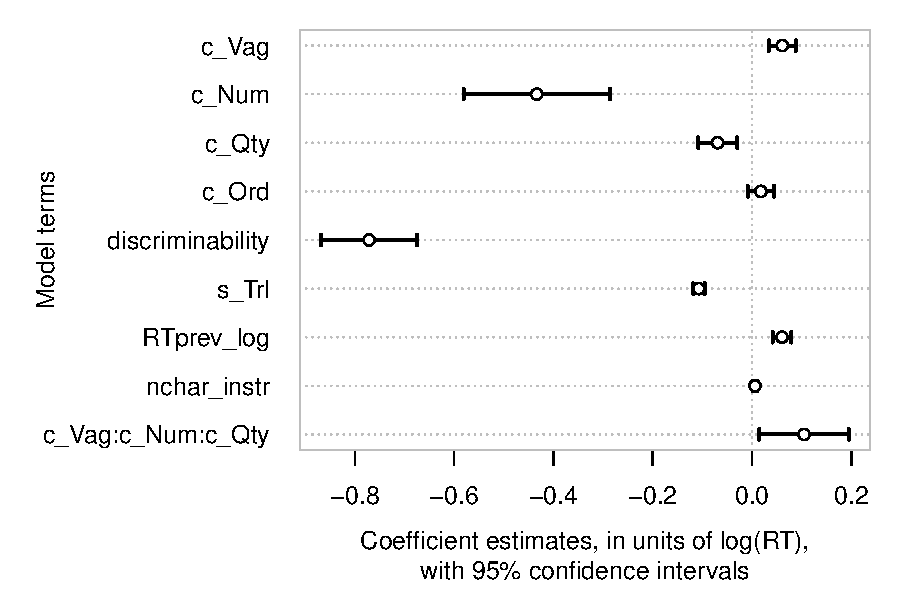
\includegraphics[width=\maxwidth]{figure/graphics-plotModelCoefsAndCis-1} 

}

\caption[Coefficient estimates and their (Wald) 95 per cent confidence intervals]{Coefficient estimates and their (Wald) 95 per cent confidence intervals}\label{fig:plotModelCoefsAndCis}
\end{figure}


\end{knitrout}


\clearpage 

\begin{knitrout}\scriptsize
\definecolor{shadecolor}{rgb}{0.969, 0.969, 0.969}\color{fgcolor}\begin{kframe}
\begin{alltt}
\hlkwd{par}\hlstd{(}\hlkwc{mfrow} \hlstd{=} \hlkwd{c}\hlstd{(}\hlnum{2}\hlstd{,} \hlnum{4}\hlstd{))}
\hlkwd{plotLMER.fnc}\hlstd{(v5)}
\end{alltt}
\begin{verbatim}
effect size (range) for  c_Vag is  0.03470056 
effect size (range) for  c_Num is  0.4073765 
effect size (range) for  c_Qty is  0.09530422 
effect size (range) for  c_Ord is  0.0179595 
effect size (range) for  discriminability is  0.2346348 
effect size (range) for  s_Trl is  0.369093 
effect size (range) for  RTprev_log is  0.2759499 
effect size (range) for  nchar_instr is  0.05477539 
\end{verbatim}
\end{kframe}\begin{figure}[hbtp]

{\centering 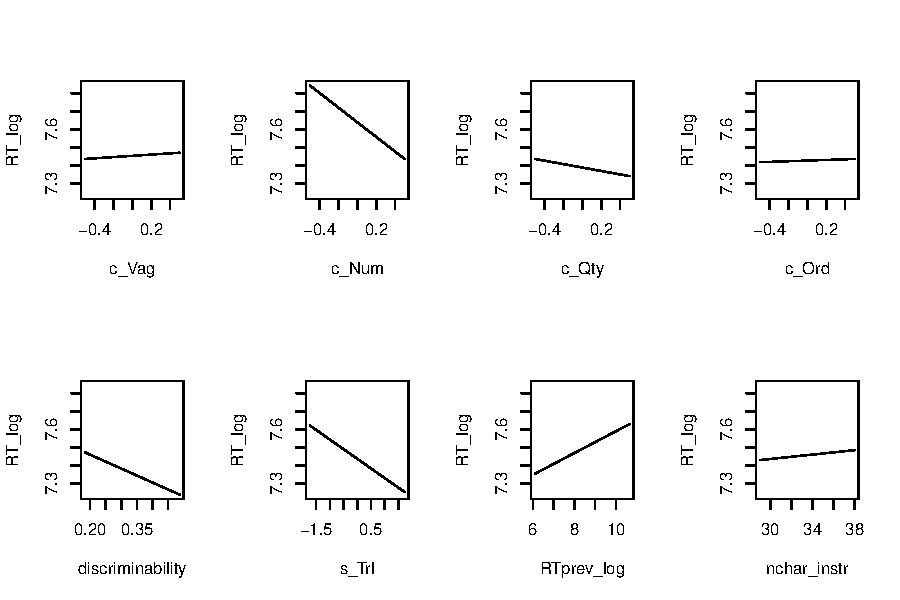
\includegraphics[width=\maxwidth]{figure/graphics-plotLMERfnc-1} 

}

\caption[plotMLERfnc]{plotMLERfnc}\label{fig:plotLMERfnc}
\end{figure}


\end{knitrout}

\clearpage

\begin{knitrout}\scriptsize
\definecolor{shadecolor}{rgb}{0.969, 0.969, 0.969}\color{fgcolor}\begin{figure}[hbtp]

{\centering 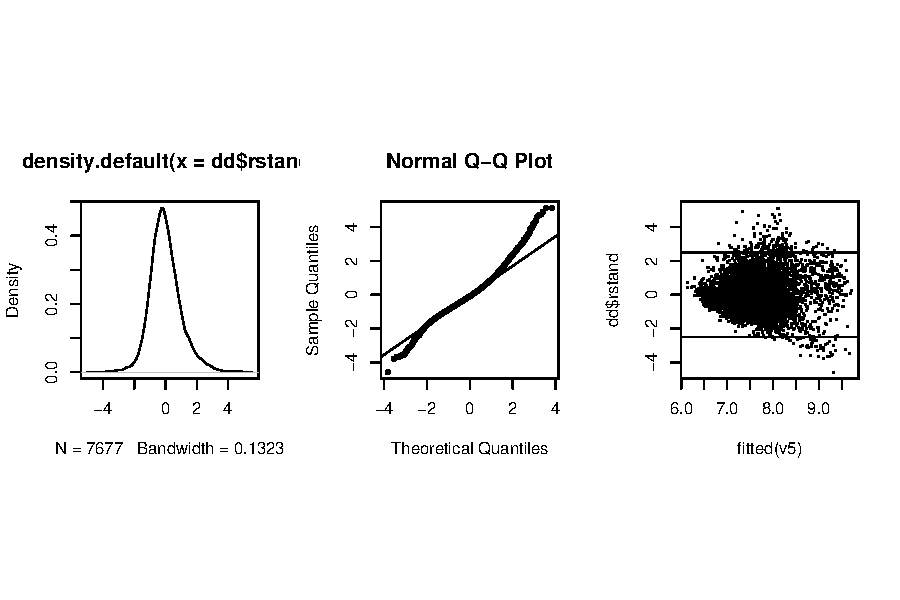
\includegraphics[width=\maxwidth]{figure/graphics-baayenPLots99-1} 

}

\caption[Baayen Model Criticism Plots]{Baayen Model Criticism Plots}\label{fig:baayenPLots99}
\end{figure}


\end{knitrout}

\clearpage

\section{lmerTest Version}

\begin{knitrout}\scriptsize
\definecolor{shadecolor}{rgb}{0.969, 0.969, 0.969}\color{fgcolor}\begin{kframe}
\begin{alltt}
\hlstd{v6} \hlkwb{<-} \hlstd{lmerTest}\hlopt{::}\hlkwd{lmer}\hlstd{(}\hlkwc{data}\hlstd{=dd,}
                     \hlstd{RT_log} \hlopt{~}
                       \hlstd{c_Vag} \hlopt{+} \hlstd{c_Num} \hlopt{+} \hlstd{c_Qty} \hlopt{+} \hlstd{c_Ord} \hlopt{+}
                       \hlstd{c_Num}\hlopt{:}\hlstd{c_Vag}\hlopt{:}\hlstd{c_Qty} \hlopt{+}
                       \hlstd{discriminability} \hlopt{+}
                       \hlstd{s_Trl} \hlopt{+}
                       \hlstd{RTprev_log} \hlopt{+}
                       \hlstd{nchar_instr} \hlopt{+}
                       \hlstd{(}\hlnum{1}\hlopt{+}\hlstd{c_Vag} \hlopt{+} \hlstd{c_Num} \hlopt{+} \hlstd{c_Qty} \hlopt{+} \hlstd{c_Ord}\hlopt{|}\hlstd{Subject))}
\end{alltt}
\end{kframe}
\end{knitrout}

\begin{knitrout}\scriptsize
\definecolor{shadecolor}{rgb}{0.969, 0.969, 0.969}\color{fgcolor}\begin{kframe}
\begin{alltt}
\hlkwd{summary}\hlstd{(v6)}
\end{alltt}
\begin{verbatim}
Linear mixed model fit by REML t-tests use Satterthwaite approximations to degrees of freedom [
lmerMod]
Formula: RT_log ~ c_Vag + c_Num + c_Qty + c_Ord + c_Num:c_Vag:c_Qty +  
    discriminability + s_Trl + RTprev_log + nchar_instr + (1 +  
    c_Vag + c_Num + c_Qty + c_Ord | Subject)
   Data: dd

REML criterion at convergence: 11474.8

Scaled residuals: 
    Min      1Q  Median      3Q     Max 
-4.5470 -0.6351 -0.0955  0.5372  5.0914 

Random effects:
 Groups   Name        Variance Std.Dev. Corr                   
 Subject  (Intercept) 0.153949 0.39236                         
          c_Vag       0.001546 0.03932   0.69                  
          c_Num       0.165314 0.40659  -0.67 -0.64            
          c_Qty       0.008148 0.09027   0.16  0.26 -0.34      
          c_Ord       0.001559 0.03949  -0.13  0.02 -0.39 -0.52
 Residual             0.249734 0.49973                         
Number of obs: 7677, groups:  Subject, 30

Fixed effects:
                    Estimate Std. Error         df t value Pr(>|t|)    
(Intercept)        7.172e+00  1.222e-01  2.370e+02  58.671  < 2e-16 ***
c_Vag              6.094e-02  1.387e-02  3.300e+01   4.393 0.000112 ***
c_Num             -4.336e-01  7.515e-02  2.900e+01  -5.770 2.97e-06 ***
c_Qty             -6.907e-02  2.005e-02  2.900e+01  -3.445 0.001743 ** 
c_Ord              1.796e-02  1.350e-02  5.100e+01   1.331 0.189164    
discriminability  -7.714e-01  4.927e-02  7.551e+03 -15.658  < 2e-16 ***
s_Trl             -1.070e-01  5.807e-03  7.558e+03 -18.421  < 2e-16 ***
RTprev_log         6.047e-02  9.692e-03  7.594e+03   6.239 4.63e-10 ***
nchar_instr        6.086e-03  1.944e-03  7.551e+03   3.131 0.001749 ** 
c_Vag:c_Num:c_Qty  1.049e-01  4.607e-02  7.551e+03   2.278 0.022742 *  
---
Signif. codes:  0 '***' 0.001 '**' 0.01 '*' 0.05 '.' 0.1 ' ' 1

Correlation of Fixed Effects:
            (Intr) c_Vag  c_Num  c_Qty  c_Ord  dscrmn s_Trl  RTprv_ nchr_n
c_Vag        0.083                                                        
c_Num       -0.369 -0.337                                                 
c_Qty        0.069  0.117 -0.278                                          
c_Ord       -0.052  0.007 -0.206 -0.228                                   
discrmnblty -0.140  0.004 -0.001  0.000  0.001                            
s_Trl       -0.114  0.003 -0.001 -0.002  0.006  0.017                     
RTprev_log  -0.607  0.006 -0.004 -0.003  0.019  0.015  0.185              
nchar_instr -0.524  0.237 -0.034  0.018  0.000  0.017  0.000  0.006       
c_Vg:c_N:_Q  0.073 -0.033  0.005 -0.003  0.000 -0.002 -0.001 -0.002 -0.138
\end{verbatim}
\end{kframe}
\end{knitrout}

\clearpage
\section{Lmer model: after outlier removal}
not done yet.
\clearpage
\section{Borderline responses}

\begin{knitrout}\scriptsize
\definecolor{shadecolor}{rgb}{0.969, 0.969, 0.969}\color{fgcolor}

{\centering 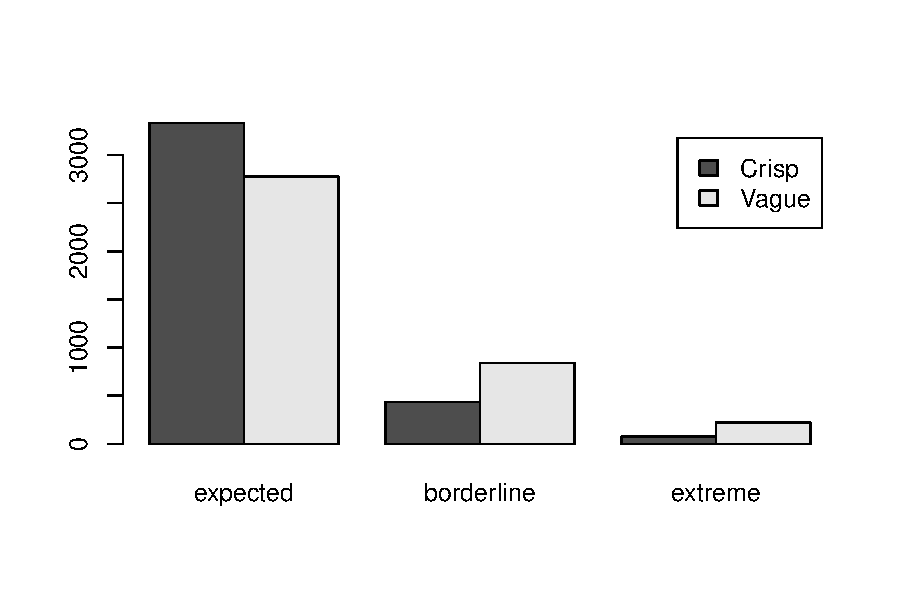
\includegraphics[width=\maxwidth]{figure/graphics-barplotBorderline-1} 

}



\end{knitrout}

% latex table generated in R 3.3.1 by xtable 1.8-2 package
% Sat Oct  1 13:19:28 2016
\begin{table}[htbp]
\centering
\begingroup\small
\begin{tabular}{rrr}
  \hline
 & Crisp & Vague \\ 
  \hline
expected & 3332 & 2776 \\ 
  borderline & 433 & 841 \\ 
  extreme &  75 & 220 \\ 
   \hline
\end{tabular}
\endgroup
\caption{Borderline cases counts} 
\end{table}


\clearpage
\appendix
\section{Functions listing}
\clearpage
\subsection{Gather Data}

\begin{knitrout}\scriptsize
\definecolor{shadecolor}{rgb}{0.969, 0.969, 0.969}\color{fgcolor}\begin{kframe}
\begin{alltt}
\hlkwd{source}\hlstd{(}\hlstr{"e2-preprocessing.R"}\hlstd{,} \hlkwc{echo} \hlstd{= T)}
\end{alltt}
\begin{verbatim}

> gatherData = function() {
+     number_of_valid_subjects = 30
+     number_of_trials_per_subject = 256
+     message("Starting to gather data")
+    .... [TRUNCATED] 

> declareImpossibleRT = function(dat) {
+     message("Starting to declare impossible RTs")
+     dat$NaType = "valid_trial"
+     dat$NaType[dat$RT_o .... [TRUNCATED] 

> removeImpossibleTrials = function(dat) {
+     message("Starting to remove impossible trials")
+     a = nrow(dat)
+     dat <- dat[complete.cases(d .... [TRUNCATED] 
\end{verbatim}
\end{kframe}
\end{knitrout}

\end{document}
